\documentclass[12pt]{article}
\usepackage{amsmath}
\usepackage{amssymb}
\usepackage[letterpaper,top=0.85in,bottom=1in,left=0.75in,right=0.75in,centering]{geometry}
%\usepackage{fancyhdr}
\usepackage{enumerate}
%\usepackage{lastpage}
\usepackage{multicol}
\usepackage{graphicx}
\usepackage{tikz}
\usetikzlibrary{calc, positioning, decorations.pathmorphing}



\reversemarginpar

%\pagestyle{fancy}
%\cfoot{}
%\lhead{Math 1560}\chead{Test \# 1}\rhead{May 18th, 2017}
%\rfoot{Total: 10 points}
%\chead{{\bf Name:}}
\newcommand{\points}[1]{\marginpar{\hspace{24pt}[#1]}}
\newcommand{\skipline}{\vspace{12pt}}
%\renewcommand{\headrulewidth}{0in}
\headheight 30pt

\newcommand{\di}{\displaystyle}
\newcommand{\abs}[1]{\lvert #1\rvert}
\newcommand{\len}[1]{\lVert #1\rVert}
\renewcommand{\i}{\mathbf{i}}
\renewcommand{\j}{\mathbf{j}}
\renewcommand{\k}{\mathbf{k}}
\newcommand{\R}{\mathbb{R}}
\newcommand{\aaa}{\mathbf{a}}
\newcommand{\bbb}{\mathbf{b}}
\newcommand{\ccc}{\mathbf{c}}
\newcommand{\dotp}{\boldsymbol{\cdot}}
\newcommand{\bbm}{\begin{bmatrix}}
\newcommand{\ebm}{\end{bmatrix}}                   
                  
\begin{document}


\author{Instructor: Sean Fitzpatrick}
\thispagestyle{empty}
\vglue1cm
\begin{center}
{\bf MATH 1565 - Tutorial \#9 Solutions}\\
\end{center}

\begin{enumerate}
  \item Consider the function $f(x)=x^4\ln(x)$.
  \begin{enumerate}
  \item State the domain of $f$ \points{1}
  
\medskip

The domain of $f$ is $(0,\infty)$ since $\ln(x)$ is undefined for $x\leq 0$.
  
  \item Determine any $x$-intercepts. (If you answered (a) correctly, you'll know why I didn't ask for a $y$-intercept). \points{1}
  
\medskip

Since $x\neq 0$ we have $f(x)=0$ when $\ln(x)=0$, giving us $x=1$. Thus, $(1,0)$ is the only intercept.
  
  \item Determine $\di \lim_{x\to 0^+}f(x)$. (Use l'Hospital's Rule.) \points{3}
  
\medskip

We have 
\[
\lim_{x\to 0^+}f(x) = \lim_{x\to 0^+}x^4\ln(x) = \lim_{x\to 0^+}\frac{\ln(x)}{x^{-4}}.
\]
This is a limit of the form ``$\infty/\infty$''. Taking the derivative of the top and bottom, we have
\[
\lim_{x\to 0^+}\frac{1/x}{-4x^{-5}} = \lim_{x\to 0^+}\frac{-1}{4}x^4 = 0.
\]
Since this limit exists, the original limit does as well, and $\di\lim_{x\to 0^+}f(x) = 0$.
  
  \item Compute $f'(x)$. \points{2}
  
 \begin{align*}
 f'(x) & = 4x^3\ln(x) + x^4(1/x)\\
 & = 4x^3\ln(x)+x^3 = x^3(4\ln(x)+1).
 \end{align*}
  
  \item Construct a sign diagram for $f'$. On what intervals is $f$ increasing/decreasing? \points{2}
  
\medskip

From above, since $x>0$, we have $f'(x)=0$ only if $4\ln(x)+1=0$, giving us $\ln(x)=-1/4$, so $x=e^{-1/4}$ is our only critical number. Since $\ln(x)$ is an increasing function, we see that $4\ln(x)+1<0$ when $x<e^{-1/4}$, and $4\ln(x)+1>0$ when $x>e^{-1/4}$. This gives the sign diagram
 \begin{center}
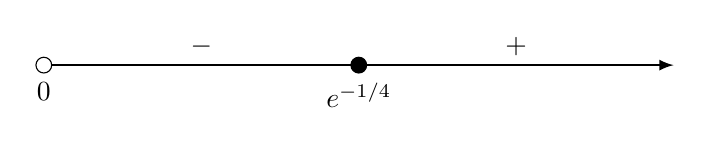
\begin{tikzpicture}[>=latex]
  \draw [thick, ->] (-4,0) -- (4,0);
  \draw [fill=white] (-4,0) circle [radius =.1];
  \draw [fill] (0,0) circle [radius =.1];
  \node at (-2,0) [above] {$-$};
  \node at (2,0) [above] {$+$};
  \node at (-4,-0.1) [below] {$0$};
  \node at (0,-0.1) [below] {$e^{-1/4}$};
  \end{tikzpicture}
\end{center}

  
  \item Classify any critical numbers found in part (e) as local maxima, minima, or neither. \points{1}
  
  \medskip
  
  From the sign diagram above, the first derivative test tells us that we have a local minimum at $(e^{-1/4},f(e^{-1/4}))$. 
  
  
  \item Compute $f''(x)$.\points{2}
  
\medskip

\begin{align*}
f''(x)&=12x^2\ln(x)+4x^3(1/x)+3x^2\\
& = 12x^2\ln(x)+7x^2 = x^2(12\ln(x)+7).
\end{align*}
  
  \item Construct a sign diagram for $f''$.  On what intervals is the graph of $f$ concave up/down? \points{2}
  
\medskip

Using the same reasoning that we used to obtain the sign diagram for $f'(x)$, we see that $f''(x)=0$ for $x=e^{-7/12}$, and we get the sign diagram
 \begin{center}
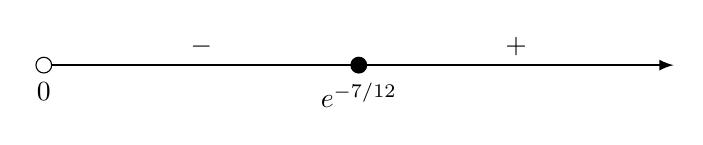
\begin{tikzpicture}[>=latex]
  \draw [thick, ->] (-4,0) -- (4,0);
  \draw [fill=white] (-4,0) circle [radius =.1];
  \draw [fill] (0,0) circle [radius =.1];
  \node at (-2,0) [above] {$-$};
  \node at (2,0) [above] {$+$};
  \node at (-4,-0.1) [below] {$0$};
  \node at (0,-0.1) [below] {$e^{-7/12}$};
  \end{tikzpicture}
\end{center}
  
  \item Determine any inflection points on the graph of $f$. \points{1}
  
  \medskip
  
  From the above sign diagram, we see that there is an inflection point at $(e^{-7/12},f(e^{-7/12}))$. 
  
  \item Sketch the graph of $f$. Your graph should reflect your results in parts (a) - (i) above. Label any intercepts, critical points, and inflection points.\points{3}
  
  \medskip
  
  Our graph does not need to be to scale (and indeed, if we want to see the features noted above, we need to stretch the $y$ scale). The precise location of the critical point and inflection point are not important, as long as we note that $e^{-7/12}<e^{-1/4}$ and $f(e^{-7/12})>f(e^{-1/4})$, so the inflection point is above and to the left of the critical point. Using all the information above, we get the following graph:
  \begin{center}
  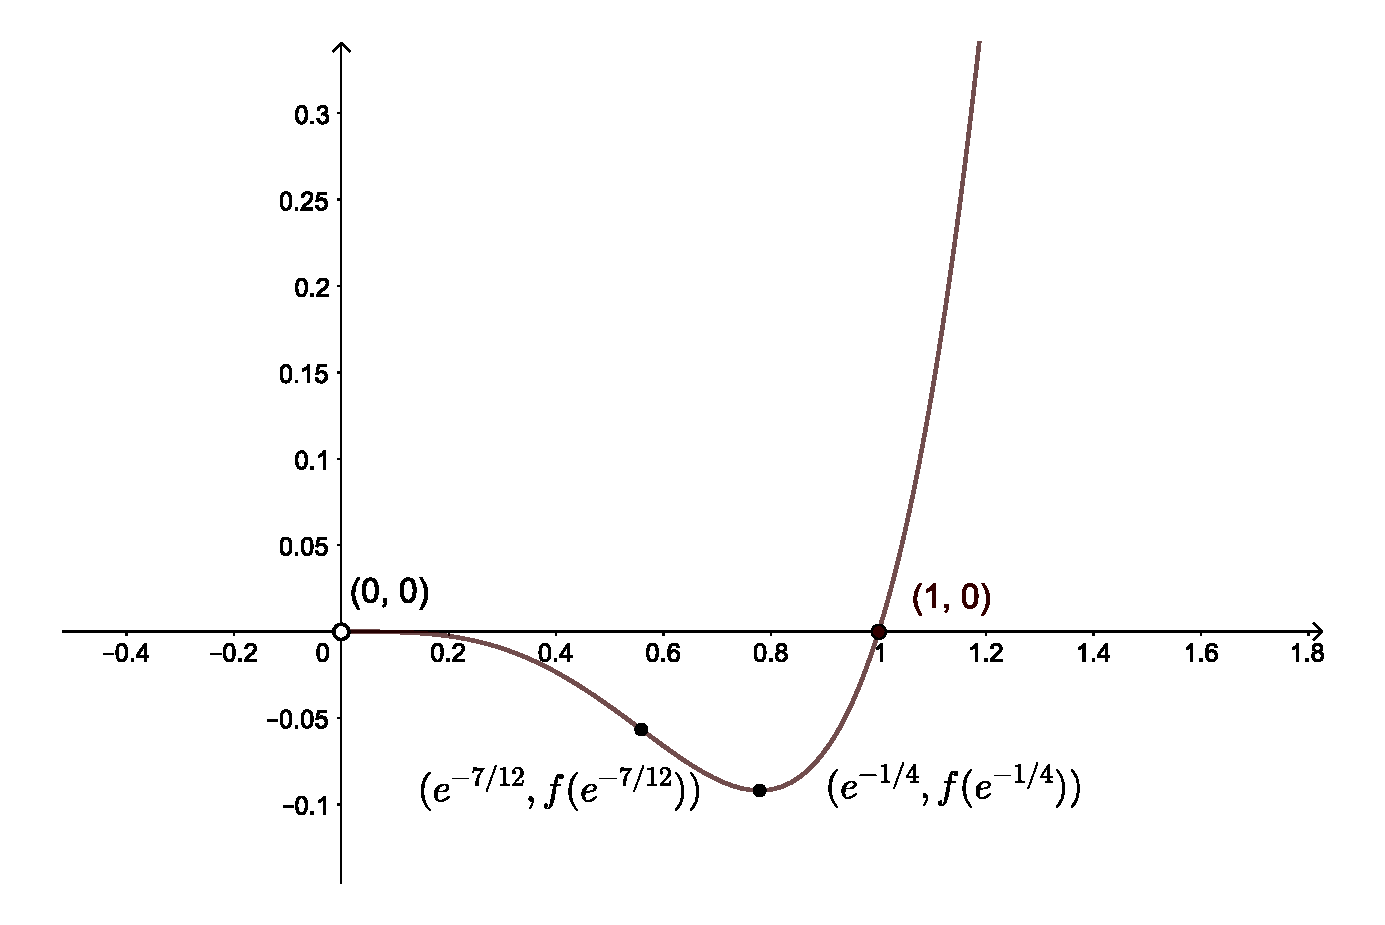
\includegraphics[width=4in]{Tut09Graph}
  \end{center}
  \end{enumerate}
\end{enumerate}
\end{document}